\question{Движение одиночного заряда в скрещенных однородных статических
  электрическом и магнитном полях}

Рассмотрим траектории движения заряженных частиц, когда они попадают в 
область, где существуют взаимно перпендикулярные электростатическое 
\( \vec{E}_0 \) и магнитное \( \vec{B}_0 \) поля. Ориентация вектора магнитной 
индукции \( \vec{B}_0 = \vec{i}B_0 \), а вектора напряженности электрического 
поля \( \vec{E}_0 = -\vec{j}E_0 \). Будем считать, что электрическое поле
создается системой из двух пластин, бесконечно протяженных в плоскостях
\( x0z \) и \( xdz \), между которыми приложена разность потенциалов \( U_0 \),
распределение потенциала в области между пластинами 
\( U(y) = U_0 \frac{y}{d} \), а напряженность электрического поля 
\( E_0 = \frac{U_0}{d} \).

\begin{figure}[h!]
	\center
	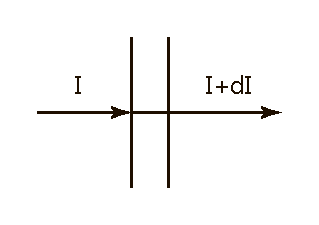
\includegraphics[width=.4\textwidth]{07_01}
	\caption{Пространство со скрещенными полями}
	\label{img07.1}
\end{figure}

Уравнение движения при нерелятивистских скоростях частицы имеет вид
\[
	m_0 \ddot{\vec{R}} = q\vec{E}_0 + q\left[ \vec{v}\vec{B}_0 \right]
\]

Рассмотрим его относительно составляющих по координатам 
\( x \), \( y \), \( z \):
\begin{equation}
	\left. \begin{array}{c}
		\ddot{x} = 0 \\
		\ddot{y} = -\frac{q}{m_0}E_0 + \frac{q}{m_0}B_0 \dot{z} \\
		\ddot{z} = -\frac{q}{m_)}B_0 \dot{y}
	\end{array} \right\}
	\label{eq07.2.65}
\end{equation}

Если частица на входе в систему не имеет составляющей скорости вдоль \( 0x \), 
то ее координата по \( x \) не меняется и траектория будет лежать только в 
плоскости \( у0z \). Для простоты положим, что на влете в систему 
\( x\Big|_{t=0} = 0\), \( \dot{x}\Big|_{t=0} = 0 \), поэтому будем 
рассматривать только два последних уравнения (\ref{eq07.2.65}). Их решение 
можно искать различными путями. Выберем следующий. Проинтегрируем один раз 
по времени последнее уравнение из системы (\ref{eq07.2.65}):
\begin{equation}
	\dot{z} = -\omega_c y + A
	\label{eq07.2.66}
\end{equation}

Если положить начальные условия на влёте частицы в рассматриваемую область в 
виде \( y\Big|_{t=0} = y_0 \), \( z\Big|_{t=0} = 0 \), 
\( \dot{y}\Big|_{t=0} = v_{0y} \), \( \dot{z}\Big|_{t=0} = v_{0z} \), то 
постоянная
\begin{equation}
	A = v_{0z} + \omega_c y_0
	\label{eq07.2.67}
\end{equation}

Подставим полученное решение (\ref{eq07.2.66}) во второе уравнение системы 
(\ref{eq07.2.65}):
\[
	\ddot{y} + \omega^2_c y = -\frac{q}{m_0} E_0 + \omega_c A = 
		-\omega_c u_0 + \omega_c A
\]

где \( u_0 = E_0 / B_0 \) -- переносная скорость электрона. Решение этого 
неоднородного уравнения

\begin{equation}
	y = G\sin\omega_c t + D\cos\omega_c t + \frac{1}{\omega_c}( A - u_0 )
	\label{eq07.2.68}
\end{equation}

а постоянные интегрирования \( D \) и \( G \) определяются из введенных 
начальных условий:

\begin{equation}
	D = y_0 - \frac{1}{\omega_c}( A - u_0 ); \quad
	G = \frac{v_{0y}}{\omega_c}
	\label{eq07.2.69}
\end{equation}

Зависимость \( z(t) \) определим, подставив в (\ref{eq07.2.66}) решение 
(\ref{eq07.2.68}) и проинтегрировав (\ref{eq07.2.66}) по \( t \):
\begin{equation}
	z = G\cos\omega_c t - D\sin\omega_c t + A + C
	\label{eq07.2.70}
\end{equation}

Постоянная интегрирования
\begin{equation}
	C = -G = -\frac{v_{0y}}{\omega_c}
	\label{eq07.2.71}
\end{equation}

Подставляя (\ref{eq07.2.67}), (\ref{eq07.2.69}), (\ref{eq07.2.71}) в выражения 
(\ref{eq07.2.68}) и (\ref{eq07.2.70}), после несложных преобразований 
получаем зависимости \( y(t) \), \( z(t) \):
\begin{equation}
	\left. \begin{array}{c}
		y = y_0 + \frac{v_{0y}}{\omega_c}\sin\omega_c t +
			\frac{u_0-v_{0z}}{\omega_c}(\cos\omega_c t - 1) \\
		z = \frac{v_{0y}}{\omega_c}(\cos\omega_c t - 1 ) - 
			\frac{u_0-v_{0z}}{\omega_c}\sin\omega_c t + u_0 t
	\end{array} \right\}
	\label{eq07.2.72}
\end{equation}

Из (\ref{eq07.2.72}) легко получить параметрическую зависимость
\begin{equation}
	\left[ y - y_0 + \frac{1}{\omega_c}(u_0 - v_{0z} \right]^2 + 
		\left[ z + \frac{v_{0y}}{\omega_c} - u_0 t \right]^2 = 
		\frac{v^2_{0y} + (u_0 - v_{0z})^2}{\omega^2_c}
	\label{eq07.2.73}
\end{equation}
из которой следует, что частица в скрещенных статистических полях движется по 
окружности с радиусом
\begin{equation}
	R = \frac{1}{|\omega_c|}\sqrt{v^2_{0y}+(u_0 -v_{0z})^2}
	\label{eq07.2.74}
\end{equation}
вокруг центра с изменяющимися во времени координатами:
\begin{equation}
	\left. \begin{array}{c}
		y = y_0 - \frac{1}{\omega_c}(u_0 - v_{0z}) \\
		z = u_0 t - \frac{v_{0z}}{\omega_c}
	\end{array} \right\}
	\label{eq07.2.75}
\end{equation}
Центр окружности перемещается вдоль оси \( 0z \) с постоянной скоростью 
\( u0 \).

Из (\ref{eq07.2.72}) или (\ref{eq07.2.73}) можно выделить ряд интересных 
частных случаев. 

1. Пусть \( y_0 = v_0 = v_{0z} = 0 \). Тогда
\begin{equation}
	\left. \begin{array}{c}
		y = \frac{u_0}{\omega_c}(\cos\omega_t - 1) \\
		z = \frac{u_0}{\omega_c}(\omega_c t - \sin\omega_c t)
	\end{array} \right\}
	\label{eq07.2.76}
\end{equation}

Система (\ref{eq07.2.76})  описывает циклоиду  (рис. \ref{img07.2}), 
представляющую собой след точки, лежащей на ободе колеса радиуса 
\( R_\text{окр} = u_0 / \omega_c \), катящегося вдоль оси \( 0z \) со 
скоростью \( u_0 \). На (рис.\ref{img07.2}) тонкой пунктирной линией 
нарисована траектория частицы с отрицательным зарядом (\( q < 0 \), 
\( \omega_c < 0 \)). При \( q > 0 \) картина будет иметь такой же вид, если 
изменить знаки у \( E_0 \) и \( B_0 \). Очевидно, что при выполнении условия 
\( d = 2u_0/\omega_c \) частица попадает на верхнюю плоскость. Это условие, 
приводящее к соотношению
\[
	B_{0\text{кр}} = \frac{1}{d}\sqrt{2\left| \frac{m_0}{q} \right| U_0}
\]
определяет критическую величину магнитной индукции, при которой еще возможна 
циклоидальная траектория частицы.

\begin{figure}[h!]
	\center
	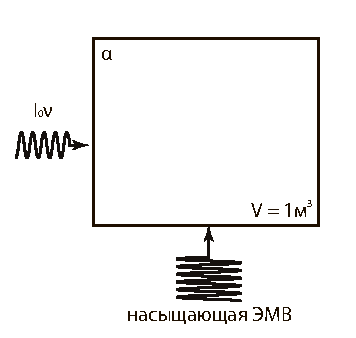
\includegraphics[width=.4\textwidth]{07_02}
	\caption{Траектории частиц в скрещенных полях: \\
		-- -- уравнение (\ref{eq07.2.76}); --- --- уравнение 
		(\ref{eq07.2.77}); --- уравнение (\ref{eq07.2.78})}
	\label{img07.2}
\end{figure}

2. Интересен случай, когда \( y = 0 \), \( v_{0y} = 0 \), \( v_{0z} = u_0 \) 
то есть частица влетает в область параллельно плоскостям со скоростью 
\( u_0 \). В этом случае из (\ref{eq07.2.72}) находим:

\begin{equation}
	y = y_0; \quad
	z = u_0 t
	\label{eq07.2.77}
\end{equation}
то есть траектория частицы представляет собой прямую линию. Это соответствует 
случаю, когда частица находится в центре колеса (штриховая линия 
на рис.\ref{img07.2}).

3. В случае, когда \( v_{0y} = 0 \), а \( v_{0z} \neq u_0\), из 
(\ref{eq07.2.78}) следует, что
\begin{equation}
	\left. \begin{array}{c}
		y = \frac{u_0-v_{0z}}{\omega_c}(\cos\omega_c t - 1) \\
		z = ut - \frac{u_0-v_{0z}}{\omega_c}\sin\omega_c t
	\end{array} \right\}
	\label{eq07.2.78}
\end{equation}
и траектория частицы представляет собой трохоиду (кривая, нарисованная 
сплошной линией на рис.\ref{img07.2}).